\documentclass{beamer}
\usetheme{Warsaw}
\usetheme{CambridgeUS}
\usefonttheme{structuresmallcapsserif}
\usefonttheme{serif}
\useinnertheme{circles}

\setbeamertemplate{background canvas}[vertical shading][bottom=white,top=white]   
\setbeamercolor{math text}{fg=black!10!Lublue}
\setbeamercolor{block title}{bg=blue!40!white, fg=black}
%\setbeamertemplate{navigation symbols}{}
\setbeamerfont{frametitle}{size=\normalsize}

\definecolor{light-gray}{gray}{0.99}
\definecolor{light-blue}{rgb}{0.90,0.90,0.98}
\definecolor{light-yellow}{rgb}{0.95,0.95,0.10}
\definecolor{dark-green}{rgb}{0.10,0.50,0.10}
\definecolor{Lublue}{rgb}{.10,.10,.70}
\definecolor{links}{rgb}{0.05,0.05,0.95}
\hypersetup{colorlinks,linkcolor=,urlcolor=links}

\definecolor{UNAMoro}{rgb}{0.796, 0.671, 0.341} % (secondary)
\definecolor{UNAMblue}{rgb}{0.067, 0.129, 0.275} % (primary)

%\setbeamercolor{palette primary}{bg=UNAMblue,fg=white}
%\setbeamercolor{palette secondary}{bg=UNAMblue,fg=white}
\setbeamercolor{palette tertiary}{bg=UNAMblue,fg=white}
%\setbeamercolor{palette quaternary}{bg=UNAMblue,fg=white}
\setbeamercolor{structure}{fg=UNAMblue} % itemize, enumerate, etc
\setbeamercolor{section in toc}{fg=UNAMblue} % TOC sections
\setbeamercolor{subsection in toc}{fg=Lublue} % TOC sections
% Override palette coloring with secondary
\setbeamercolor{subsection in head/foot}{bg=UNAMoro,fg=UNAMblue}
\setbeamercolor{frametitle}{bg=UNAMoro,fg=UNAMblue}
\setbeamercolor{subtitle}{bg=UNAMoro,fg=UNAMblue}

\usepackage[utf8]{inputenc}
\usepackage[spanish]{babel}
\usepackage{amsmath}
\usepackage{amsfonts}
\usepackage{amssymb}
\usepackage{empheq}
\usepackage{graphicx}
\usepackage{color}
\usepackage{listings}
\usepackage{hyperref}
\usepackage{wasysym}
\usepackage{alltt}
\usepackage{algorithmic}
\usepackage{cancel}
\usepackage[export]{adjustbox}
\usepackage{caption}
\usepackage{tikz}
\usetikzlibrary{arrows,backgrounds}
\tikzstyle{block}=[draw opacity=0.7,line width=1.4cm]

\graphicspath{{./Figuras/}{../Figuras/}}


%%%%%%%%%%%%%%%%%%%%%%%%%%%%%% User specified LaTeX commands.
\newcommand{\Vector}[1]{{\mathbf{#1}}}
\newcommand{\Tensor}[1]{\underline{\underline{\mathbf{#1}}}}
\newcommand*\widefbox[1]{\fbox{\hspace{1em}#1\hspace{1em}}}
%%%%%%%%%%%%%%%%%%%%%%%%%%%%%%
% Definimos el punto decimal.
\spanishdecimal{.}
%%%%%%%%%%%%%%%%%%%%%%%%%%%%%%

% the beginning of each subsection:
\AtBeginSection[]
{
	\begin{frame}<beamer>{Contenido}
		\tableofcontents[currentsection]
	\end{frame}
}

\title[PAPIME--PE101019]{Diferencias Finitas}   
\subtitle{Problemas estacionarios II}

\author[\copyright LMCS]{ \textcolor{UNAMblue}{Modelación computacional en las ciencias y las ingenierías como apoyo en el proceso enseñanza-aprendizaje\\(PAPIME-PE101019)}} 
\institute[IGEF--UNAM] 
{ 
	{\small{Instituto de Geof\'isica}} \\ 
	\vspace{0.15cm}
	{\small{Universidad Nacional Aut\'onoma de M\'exico}} \\
	\vspace{0.15cm}
	
\includegraphics[height=.85cm]{unamlogo.png} 
}

\date[2019--2021]{\\ {\tiny{Esta obra está bajo una 
			\href{https://creativecommons.org/licenses/by-nc-sa/4.0/}{Licencia Creative Commons Atribución-NoComercial-CompartirIgual 4.0 Internacional.}}\\
		
\includegraphics[scale=0.20]{ccPyNoxtli.png}}}

% To uncover everything in a step-wise fashion:
%\beamerdefaultoverlayspecification{<+->}

\begin{document}
	
\begin{frame}
\titlepage
\end{frame}

\begin{frame}{Contenido}
\tableofcontents
\end{frame}

\section{Calibración 1.}

\begin{frame}{Modelo Matemático}
	
Considere el siguiente problema:
	\begin{eqnarray}
		\frac{d^2 T(x)}{d x^2} + \omega ^2 T(x) & = & 0 \,\,\,\,\, x \in [0,1] \label{eq:cal01}\\
		T(0) & = & 1 \nonumber\\
		T(1) & = & 1 \nonumber
	\end{eqnarray}
	
cuya soluci\'on anal\'itica es:
$\displaystyle T(x) = \frac{1-\cos(\omega)}{\sin(\omega)} \sin(\omega x) + \cos(\omega x)$
	
\strut
	
donde $\omega$ = constante. 
	
\end{frame}


\begin{frame}{Modelo Numérico}
	
{\small 
Recordemos que la segunda derivada se puede aproximar como sigue (véase la figura como referencia):
\begin{equation}\label{eq:segundaDer1D}
\boxed{
	\left.\frac{d^2 T}{d x^2}\right|_i = \frac{T_{i+1} - 2 T_{i} + T_{i-1}}{h^2} + \mathcal{O}(h^2)
}
\end{equation}
$$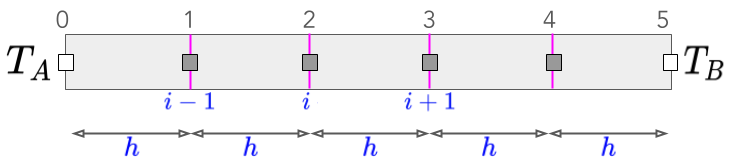
\includegraphics[scale=0.30]{ModCon05.png}$$	
%	
Usando \eqref{eq:segundaDer1D} en \eqref{eq:cal01} obtenemos
\[
\frac{T_{i+1} - 2 T_{i} + T_{i-1}}{h^2} + \omega T_{i} = 0
\]
%
que podemos escribir como:
\[
- T_{i+1} + (2 - \omega / r_i) T_{i} - T_{i-1} = 0 
\]

donde $\displaystyle r_i = \frac{\kappa_i}{h^2}$ y en este caso $\kappa_i = 1, \, \forall i$.
}
\end{frame}

\begin{frame}{Modelo Numérico}

El sistema lineal para este caso, para cualquier $N$, es:
	
{\scriptsize 
\[ 
\underbrace{
	\left[
	\begin{matrix}
	2-\omega/r & -1 & 0 & 0 & \dots & 0  \\
	-1 & 2-\omega/r & -1 & 0 & \dots & 0  \\
	0 & -1 & 2-\omega/r & -1 & \dots & 0  \\
	\vdots & \ddots & \ddots & \ddots & \ddots & \vdots \\
	0 & \dots & 0 & -1 & 2-\omega/r & -1   \\
	0 & \dots & 0 & 0 & -1 & 2-\omega/r    
	\end{matrix}
	\right]}_{\Tensor{A}_{N \times N}}
\underbrace{
	\left[
	\begin{matrix}
	T_1 \\ T_2 \\ T_3 \\ \vdots \\ T_{N-1} \\ T_N
	\end{matrix}
	\right]}_{\Vector{T}_N} =
\underbrace{
	\frac{1}{r}
	\left[
	\begin{matrix}
	S_1 \\ S_2 \\ S_3 \\ \vdots \\ S_{N-1} \\ S_N
	\end{matrix}
	\right] +
	\left[
	\begin{matrix}
	T_A \\ 0 \\ 0 \\ \vdots \\ 0 \\ T_B
	\end{matrix}
	\right]}_{\Vector{b}_N}
\]
}

donde $\displaystyle r = \frac{\kappa}{h^2}$ y $S_i = 0, \, \forall i$.
\end{frame}

\subsection{Ejercicio 3.}

\begin{frame}

\begin{exampleblock}{Ejercicio 3.}
	\begin{enumerate}
		\item Resuelva el problema numéricamente usando diferencias finitas.
	\end{enumerate}
\end{exampleblock}

\end{frame}



\section{Calibración 2: Condiciones tipo Neumman}

\begin{frame}{Modelo Matemático}

Considere el siguiente problema:
		
\begin{eqnarray*}
	\frac{d^2 u(x)}{d x^2} & = & e^x \,\,\,\,\, x \in [0,1] \\
	\frac{du}{d n}(0) & = & 0 \\
	u(1) & = & 3
\end{eqnarray*}
		
cuya soluci\'on anal\'itica es:
$\displaystyle u(x) = e^x - x - e + 4 $

\strut

A continuación mostramos cuatro aproximaciones que se pueden usar para 
incorporar las condiciones de tipo Neumman en el sistema lineal.
\end{frame}

\subsection{Aproximación I.}

\begin{frame}{Aproximación de primer orden, sistema de $(N+1) \times (N+1)$}
	
$$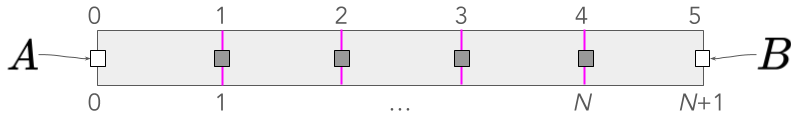
\includegraphics[scale=0.30]{ModCon06.png}$$

\begin{footnotesize}
\begin{columns}
	\begin{column}{0.45\textwidth}
		$ u_0  = A $
		
		$u_{0} - 2 u_{1} + u_{2} = r^{-1} f_1$ 
		
		$\Rightarrow \boxed{-2 u_{1} + u_{2} = r^{-1} f_1 - A}$
	\end{column}
	\begin{column}{0.5\textwidth}
		$\left.\displaystyle \frac{\partial u}{\partial n}\right|_{N+1}  = B \Longrightarrow \dfrac{u_{N+1} - u_{N}}{h} = B$ 
		
		$\Longrightarrow \boxed{\textcolor{red}{- u_{N} + u_{N+1} = h B}}$
	\end{column}
\end{columns}

\strut

\[
\Longrightarrow
\underbrace{
	\left[
	\begin{matrix}
	-2 & 1 & 0  & \dots & 0 & 0  \\
	1 & -2 & 1  & \dots & 0 & 0 \\
	\vdots & \ddots & \ddots & \ddots & \vdots & \vdots \\
	0 & \dots & 1 & -2 & 1 & 0 \\
	0 & \dots & 0 & 1 & -2 & 1 \\
	0 & \dots & 0 & 0 & \textcolor{red}{-1} & \textcolor{red}{1}        
	\end{matrix}
	\right] 
}_{(N+1) \times (N+1)}
\left[
\begin{matrix}
u_1 \\ u_2 \\ \vdots \\ u_{N-1} \\ u_N \\ u_{N+1}
\end{matrix}
\right]= 
\frac{1}{r}\left[
\begin{matrix}
f_1 \\ f_2 \\ \vdots \\ f_{N-1} \\ f_N \\ 0
\end{matrix}
\right] +
\left[
\begin{matrix}
-A \\ 0 \\  \vdots \\ 0 \\ 0 \\ \textcolor{red}{hB}
\end{matrix}
\right]
\]

donde $f(x) = e^x$, por lo tanto $f(x_i) = f_i = e^{x_i}$
\end{footnotesize}
	
\end{frame}

\subsection{Aproximación II.}

\begin{frame}{Aproximación de primer orden, sistema de $N \times N$}
	
	$$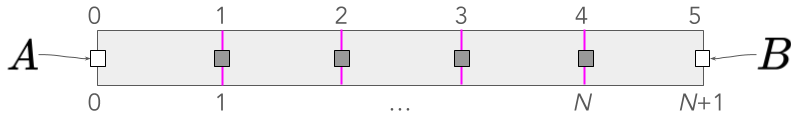
\includegraphics[scale=0.30]{ModCon06.png}$$
	
	\begin{footnotesize}
		\begin{columns}
			\begin{column}{0.45\textwidth}
				$ u_0  = A $
				
				$u_{0} - 2 u_{1} + u_{2} = r^{-1} f_1$ 
				
				$\Rightarrow \boxed{-2 u_{1} + u_{2} = r^{-1} f_1 - A}$
			\end{column}
			\begin{column}{0.5\textwidth}
				$\left.\displaystyle \frac{\partial u}{\partial n}\right|_{N+1}  = B \Longrightarrow \boxed{\textcolor{red}{u_{N+1}} = h B + u_{N}}$  
				
				$u_{N-1} - 2 u_{N} + \textcolor{red}{u_{N+1}} = r^{-1} f_N$
				
				$\Rightarrow \boxed{\textcolor{red}{u_{N-1} - u_{N} = r^{-1} f_N - hB}}$
			\end{column}
		\end{columns}
		
		\vspace{0.25cm}
		
		\[
		\Longrightarrow
		\underbrace{
			\left[
			\begin{matrix}
			-2 & 1 & 0 & 0 & \dots & 0  \\
			1 & -2 & 1 & 0 & \dots & 0  \\
			0 & 1 & -2 & 1 & \dots & 0  \\
			\vdots & \ddots & \ddots & \ddots & \ddots & \vdots \\
			0 & 0 & 0 & 1 & -2 & 1   \\
			0 & 0 & 0 & 0 & \textcolor{red}{1} & \textcolor{red}{-1}    
			\end{matrix}
			\right] }_{N \times N}
		\left[
		\begin{matrix}
		u_1 \\ u_2 \\ u_3 \\ \vdots \\ u_{N-1} \\ u_N
		\end{matrix}
		\right]= 
		\frac{1}{r} \left[
		\begin{matrix}
		f_1 \\ f_2 \\ f_3 \\ \vdots \\ f_{N-1} \\ f_N
		\end{matrix}
		\right] +
		\left[
		\begin{matrix}
		-A \\ 0 \\ 0 \\ \vdots \\ 0 \\ \textcolor{red}{-hB}
		\end{matrix}
		\right]
		\]
		
	\end{footnotesize}
	
\end{frame}

\subsection{Aproximación III.}

\begin{frame}{Aproximación de segundo orden usando tres puntos}
	
	$$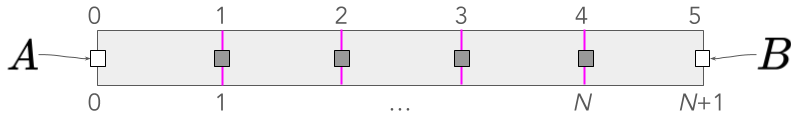
\includegraphics[scale=0.30]{ModCon06.png}$$
	
	\begin{footnotesize}
		\begin{columns}
			\begin{column}{0.40\textwidth}
				$ u_0  = A $.
				
				$u_{0} - 2 u_{1} + u_{2} = r^{-1} f_1$ 
				
				$\Rightarrow \boxed{-2 u_{1} + u_{2} = r^{-1} f_1 - A}$
			\end{column}
			\begin{column}{0.6\textwidth}
				$\left.\displaystyle \frac{\partial u}{\partial n}\right|_{N+1}  = 
				\boxed{\textcolor{red}{\frac{1}{h}\left(\frac{1}{2} u_{N-1} - 2 u_{N} + \frac{3}{2} u_{N+1}\right) = B}}$
				
			\end{column}
		\end{columns}
		
		\vspace{0.25cm}
		
		\[
		\Longrightarrow
		\underbrace{
			\left[
			\begin{matrix}
			-2 & 1 & 0  & \dots & 0 & 0  \\
			1 & -2 & 1  & \dots & 0 & 0 \\
			\vdots & \ddots & \ddots & \ddots & \vdots & \vdots \\
			0 & \dots & 1 & -2 & 1 & 0 \\
			0 & \dots & 0 & 1 & -2 & 1 \\
			0 & \dots & 0 & \textcolor{red}{\frac{1}{2}} & \textcolor{red}{-2} & \textcolor{red}{\frac{3}{2}}        
			\end{matrix}
			\right] 
		}_{(N+1) \times (N+1)}
		\left[
		\begin{matrix}
		u_1 \\ u_2 \\ \vdots \\ u_{N-1} \\ u_N \\ u_{N+1}
		\end{matrix}
		\right]= 
		\frac{1}{r} \left[
		\begin{matrix}
		f_1 \\ f_2 \\ \vdots \\ f_{N-1} \\ f_N \\ 0
		\end{matrix}
		\right] +
		\left[
		\begin{matrix}
		-A \\ 0 \\  \vdots \\ 0 \\ 0 \\ \textcolor{red}{hB}
		\end{matrix}
		\right]
		\]
		
		
	\end{footnotesize}
	
\end{frame}

\subsection{Aproximación IV.}

\begin{frame}{Aproximación de segundo orden con diferencias centrales}
	
	$$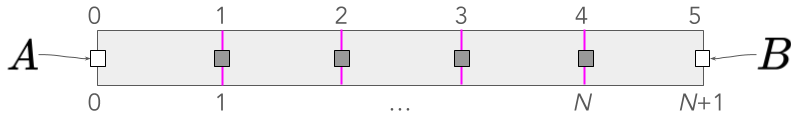
\includegraphics[scale=0.30]{ModCon06.png}$$
	
	\begin{footnotesize}
		\begin{columns}
			\begin{column}{0.35\textwidth}
				$ u_0  = A $.
				
				$u_{0} - 2 u_{1} + u_{2} = r^{-1} f_1$ 
				
				$\Rightarrow \boxed{-2 u_{1} + u_{2} = r^{-1} f_1 - A}$
			\end{column}
			\begin{column}{0.65\textwidth}
				$u_{N} - 2u_{N+1} + \textcolor{red}{u_{N+2}} = r^{-1} f_{N+1}$
				
				$\left.\displaystyle \frac{\partial u}{\partial n}\right|_{N+1}  = 
				\dfrac{\left( u_{N+2} - u_{N} \right)}{2h} = B$ 
				$\Longrightarrow  \textcolor{red}{u_{N+2} = 2hB + u_{N}}$
				
				$\Longrightarrow \boxed{\textcolor{red}{u_{N} - u_{N+1} = \frac{1}{2r} f_{N+1} - hB}}$
			\end{column}
		\end{columns}
		
		%\vspace{0.25cm}
		
		\[
		\Longrightarrow
		\underbrace{
			\left[
			\begin{matrix}
			-2 & 1 & 0  & \dots & 0 & 0  \\
			1 & -2 & 1  & \dots & 0 & 0 \\
			\vdots & \ddots & \ddots & \ddots & \vdots & \vdots \\
			0 & \dots & 1 & -2 & 1 & 0 \\
			0 & \dots & 0 & 1 & -2 & 1 \\
			0 & \dots & 0 & 0 & \textcolor{red}{1} & \textcolor{red}{-1}        
			\end{matrix}
			\right] 
		}_{(N+1) \times (N+1)}
		\left[
		\begin{matrix}
		u_1 \\ u_2 \\ \vdots \\ u_{N-1} \\ u_N \\ u_{N+1}
		\end{matrix}
		\right]= 
		\frac{1}{r} \left[
		\begin{matrix}
		f_1 \\ f_2 \\ \vdots \\ f_{N-1} \\ f_N \\ \textcolor{red}{f_{N+1}/2}
		\end{matrix}
		\right] +
		\left[
		\begin{matrix}
		-A \\ 0 \\  \vdots \\ 0 \\ 0 \\ \textcolor{red}{-hB}
		\end{matrix}
		\right]
		\]
		
	\end{footnotesize}
	
\end{frame}

%\begin{frame}{Medici\'on del error}
%	
%	\begin{itemize}
%		\item Si $\hat{u}(x)$ representa la soluci\'on exacta del problema, definimos el error en el punto $x_i$ de la aproximaci\'on como $E_i = u(x_i) - \hat{u}(x_i)$. 
%		
%		\item El vector $\Vector{E} = (E_0, E_1, \dots, E_{N+1})$ representa el error en todos los puntos de la malla. La magnitud de este vector debe darnos el error global de la aproximaci\'on. 
%		
%		\item Se puede usar cualquier norma:
%		
%		\begin{itemize}
%			\item Norma infinito: $ \displaystyle
%			|| E ||_\infty = \max\limits_{1 \leq i \leq N}|E_i| = \max\limits_{1 \leq i \leq N} |u(x_i) - \hat{u}(x_i) |$
%			
%			\item Norma uno:
%			\[
%			||E||_1 = h \sum\limits_{i=1}^{N} |E_i|
%			\]
%			
%			\item Norma Euclideana:
%			\[
%			||E||_2 = \left(h \sum\limits_{i=1}^{N} |E_i|^2 \right)^{1/2}
%			\]
%		\end{itemize}
%		
%	\end{itemize}
%	
%\end{frame}

\subsection{Ejercicio 4.}

\begin{frame}
	
\begin{exampleblock}{Ejercicio 4.}
\begin{enumerate}
\item aaa
\end{enumerate}
\end{exampleblock}
	
\end{frame}	


\section{Calibración 3: conductividad variable}

\begin{frame}{Modelo Matemático y Numérico}
		
{\footnotesize 	
	%|sin(4 \pi x)|
Considere la ecuación de Poisson con $\kappa$ variable y
condiciones de frontera de tipo Dirichlet:	
	\begin{columns}
		\begin{column}{0.5\textwidth}
			\begin{equation}\label{eq:poisson1}
			\dfrac{d}{d x} \left(\kappa \dfrac{d u}{d x} \right) = f \quad \text{con} \quad \kappa = \kappa(x)
			\end{equation}
		\end{column}
		\begin{column}{0.5\textwidth}
			$$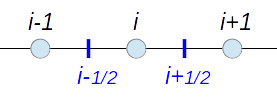
\includegraphics[scale=0.4]{malla1D_DF_Centrales.png}$$
		\end{column}
	\end{columns}
	
Definimos $\displaystyle g = \kappa \dfrac{d u}{d x}$ por lo tanto $\displaystyle \dfrac{d}{d x} \left(\kappa \dfrac{d u}{d x} \right) = \dfrac{d g}{d x}$. Esta derivada se puede aproximar como sigue (véase la figura):
	
	\begin{equation}\label{eq:poisson2}
	\dfrac{d g}{d x} \Big|_{i} = \dfrac{g_{i+\frac{1}{2}} - g_{i-\frac{1}{2}}}{h} =
	\dfrac{\left[\kappa \frac{du}{dx}\right]_{i+\frac{1}{2}} - \left[\kappa \frac{du}{dx}\right]_{i-\frac{1}{2}}}{h}
	\end{equation}
	
	\begin{equation}\label{eq:poisson3}
	\left[\kappa \frac{du}{dx}\right]_{i+\frac{1}{2}} = 
	\kappa_{i+\frac{1}{2}} \left[\dfrac{u_{i+1}-u_{i}}{h}\right] =
	\dfrac{1}{h}\left[\kappa_{i+\frac{1}{2}} u_{i+1} - \kappa_{i+\frac{1}{2}} u_{i}\right]
	\end{equation}
	
	\begin{equation}\label{eq:poisson4}
	\left[\kappa \frac{du}{dx}\right]_{i-\frac{1}{2}} = 
	\kappa_{i-\frac{1}{2}} \left[\dfrac{u_{i}-u_{i-1}}{h}\right] =
	\dfrac{1}{h}\left[\kappa_{i-\frac{1}{2}} u_{i} - \kappa_{i-\frac{1}{2}} u_{i-1}\right]
	\end{equation}
}

\end{frame}

\begin{frame}{Modelo Numérico}
	
{\footnotesize 
	
	Usando \eqref{eq:poisson2}, \eqref{eq:poisson3} y \eqref{eq:poisson4} en \eqref{eq:poisson1}
	obtenemos:
	
	\begin{equation}
	\boxed{
	\dfrac{1}{h^2} \left[
	\kappa_{i+\frac{1}{2}} u_{i+1} - 
	(\kappa_{i+\frac{1}{2}} + \kappa_{i-\frac{1}{2}}) u_{i} +
	\kappa_{i-\frac{1}{2}} u_{i-1}
	\right] = f_i
	}
	\end{equation}
	
	Condiciones de frontera tipo Dirichlet: $u_0 = A$ y $u_{N+1} = B$
	%
	\[
	\begin{array}{ccccc}
	i = 1 & \Longrightarrow &
	\kappa_{1+\frac{1}{2}} u_{2} - 
	(\kappa_{1+\frac{1}{2}} + \kappa_{1-\frac{1}{2}}) u_{1} & = & h^2 f_1 - \kappa_{1-\frac{1}{2}} A \\ \\
	i = N & \Longrightarrow &
	- (\kappa_{N+\frac{1}{2}} + \kappa_{N-\frac{1}{2}}) u_{N} +
	\kappa_{N-\frac{1}{2}} u_{N-1} & = & h^2 f_N - \kappa_{N+\frac{1}{2}} B
	\end{array}
	\]
	
	\noindent
	Donde $\kappa_{i+\frac{1}{2}}$ y $\kappa_{i-\frac{1}{2}}$ se pueden aproximar de varias maneras, por ejemplo:
	
	\[
	\begin{array}{cccc}
	\text{Promedio aritmético: } &
	\kappa_{i+\frac{1}{2}} = \dfrac{ \kappa_{i+1} + \kappa_{i}}{2} & \text{ y } &
	\kappa_{i-\frac{1}{2}} = \dfrac{ \kappa_{i-1} + \kappa_{i}}{2} \\ \\
	\text{Media armónica: } &
	\kappa_{i+\frac{1}{2}} = \dfrac{ 2 \kappa_{i+1} \kappa_{i}}{\kappa_{i+1} + \kappa_{i}} & \text{ y } &
	\kappa_{i-\frac{1}{2}} = \dfrac{ 2 \kappa_{i-1} \kappa_{i}}{\kappa_{i-1} + \kappa_{i}} 
	\end{array}
	\]
	
}
	
\end{frame}


\subsection{Ejercicio 5.}

\begin{frame}[fragile]
	
\begin{exampleblock}{Ejercicio 5.}
Reproducir los siguientes casos:
\begin{enumerate}
\item {\footnotesize $L = 1, \, N = 50, \, A = 2.0, \, B = 1.0, \, \kappa = |sin(4 \pi x)|$}
	\begin{columns}
		\begin{column}{0.5\textwidth}
			$$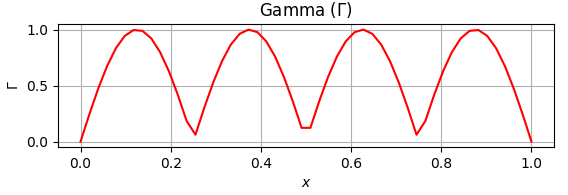
\includegraphics[width=6cm]{gamma.png}$$
		\end{column}
		\begin{column}{0.5\textwidth}  %%<--- here			
			$$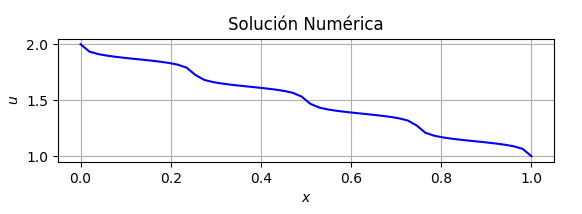
\includegraphics[width=6cm]{solucion02.png}$$
		\end{column}
	\end{columns}
	
\item {\footnotesize $L = 1, \, N = 50, \, A = 2.0, \, B = 1.0, \, \kappa = \texttt{random(x)}$}
	\begin{columns}
		\begin{column}{0.5\textwidth}
			$$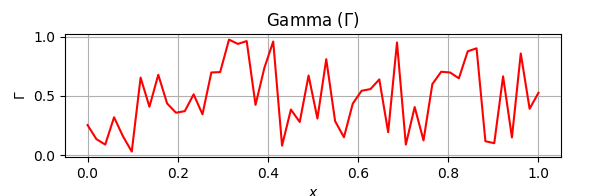
\includegraphics[width=6cm]{gamma3.png}$$
		\end{column}
		\begin{column}{0.5\textwidth}  %%<--- here			
			$$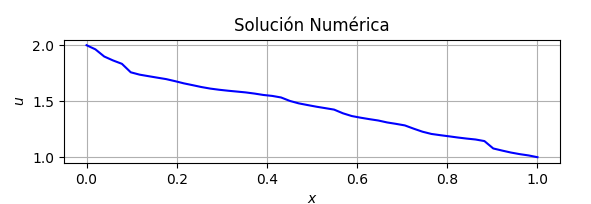
\includegraphics[width=6cm]{solucion03.png}$$
		\end{column}
	\end{columns}
\end{enumerate}
\end{exampleblock}
	
\end{frame}


\section<presentation>{Referencias}

\begin{frame}[allowframebreaks]
	%\frametitle<presentation>{Bibliograf\'{\i}a}
	
\begin{thebibliography}{10}
		
{\footnotesize 

% BOOKS 
\beamertemplatebookbibitems

\bibitem{Bergman}
[1] Bergman, T.L. and Incropera, F.P. and DeWitt, D.P. and Lavine, A.S.,
\newblock {\em Fundamentals of Heat and Mass Transfer},
\newblock Wiley, \textbf{2011}.

\bibitem{Leveque}
[2] R.J. Leveque,
\newblock {\em Finite Difference Method for Ordinary and Partial Differential Equations: Steady State and Time-Dependent Problems },
\newblock {Society for Industrial and Applied Mathematics (SIAM), Philadelphia}, \textbf{2007}.

\bibitem{Saad}
[3] Y. Saad
\newblock {\em Iterative Methods for Sparse Linear Systems}.
\newblock PWS/ITP 1996.
\newblock {Online: 
	\textsf{http://www-users.cs.umn.edu/\textasciitilde saad/books.html}, 
	\textbf{2000}}

\bibitem{Burden}
[4]  Richard Burden and J. Douglas Faires
\newblock{\em Numerical Analysis}
\newblock Cengage Learning; 9 edition (August 9, \textbf{2010})

\bibitem{Herrera1} 
[5] I. Herrera \& G. F. Pinder,
\newblock {\em Mathematical Modeling in Science and Engineering: An Axiomatic Approach}, 
\newblock John Wiley \textbf{2012}.

% ARTICULOS    
\beamertemplatearticlebibitems

%\bibitem{Delacruz2011}
%[7]   L. M. de la Cruz,
%\newblock Flujo en una y dos fases en medios porosos: modelos matemáticos, numáricos y computacionales,
%\newblock {\em Reportes técnicos del Instituto de Geofísica}, 2012-4, Agosto \textbf{2012}.


}
		
\end{thebibliography}
\end{frame}

\section{Créditos}

\begin{frame}{Créditos}
	
	\begin{center}
		\textbf{Dr. Luis M. de la Cruz Salas} \\
		\vspace{0.5cm}
		{\small{Departamento de Recursos Naturales}} \\
		\vspace{0.15cm}
		{\small{Instituto de Geof\'isica}} \\ 
		\vspace{0.15cm}
		{\small{Universidad Nacional Aut\'onoma de M\'exico}} \\
		\vspace{0.15cm}
		
\includegraphics[height=.85cm]{unamlogo.png} \\
		\vspace{1.15cm}
		{\scriptsize{Trabajo realizado con el apoyo del Programa UNAM-DGAPA-PAPIME PE101019 \\		
				
\includegraphics[scale=0.20]{ccPyNoxtli.png} }}
	\end{center}
	
\end{frame}

\end{document}
	